\documentclass[letterpaper, 10 pt, conference]{ieeeconf}
\usepackage[utf8]{inputenc}
\usepackage[ruled,algosection,vlined]{algorithm2e}
\usepackage{tikz}

\let\proof\relax
\let\endproof\relax
\usepackage{amsthm}

\usetikzlibrary{arrows,decorations,backgrounds,positioning,fit}

\IEEEoverridecommandlockouts
\overrideIEEEmargins
%\pdfobjcompresslevel=0
%\pdfminorversion=4

% See the \addtolength command later in the file to balance the column lengths
% on the last page of the document

\bibliographystyle{./IEEEtran}

\title{\LARGE \bf
On Detection of Influential Users and Content on Reddit*
}


\author{Rollen S. D'Souza$^{1}$%
  \thanks{*This work was not supported by any organization}%
  \thanks{$^{1}$Rollen S. D'Souza is a graduate student in the
    Department of Electrical and Computer Engineering,
    Faculty of Engineering,
    University of Waterloo,
    {\tt\small rollen.dsouza@uwaterloo.ca}
  }%
}

% STYLING
\theoremstyle{plain}
\newtheorem{assumption}{Assumption}[section]


\tikzset{%
  post/.style={rectangle,draw=blue!70,top color=white,bottom color=blue!20,very thick},
  user/.style={circle,top color=white,draw=red!70,bottom color=red!20,very thick},
  plain/.style={rectangle,draw=black!70,top color=white, bottom color=black!20,very thick}%
}
%

\newcommand{\red}{\color{red}}

\begin{document}
\maketitle
\thispagestyle{empty}
\pagestyle{empty}


%%%%%%%%%%%%%%%%%%%%%%%%%%%%%%%%%%%%%%%%%%%%%%%%%%%%%%%%%%%%%%%%%%%%%%%%%%%%%%%%
\begin{abstract}

%% INSERT ABSTRACT

\end{abstract}


%%%%%%%%%%%%%%%%%%%%%%%%%%%%%%%%%%%%%%%%%%%%%%%%%%%%%%%%%%%%%%%%%%%%%%%%%%%%%%%%
\section{INTRODUCTION}


\section{BACKGROUND}
{\red Talk about graph theory, centrality and Laplacians.}

\section{MODELLING}

\subsection{Assumptions}
In order to reason about influential content without temporal information or content analysis, we make the following simplifying assumptions:

\begin{assumption}
  Users are influenced (positively or negatively) by content they read.
  \label{assume:1}
\end{assumption} 

\begin{assumption}
  Users comment only on content they have read.
  \label{assume:2}
\end{assumption}

\begin{assumption}
  Content is influenced by the content creator.
  \label{assume:3}
\end{assumption}

\begin{assumption}
  Deleted users and content are not influential and do not affect other users in a meaningful way.
  \label{assume:4}
\end{assumption}

Assumptions~\ref{assume:1} and~\ref{assume:2} are the most contentious. They effectively assert that users engage with the platform in an intellectually curious manner. This is, at face value, absurd. On the other hand, the case can be made that even if users don't fully read content that they interact with, they at, the very minimum, skim and grasp the general gist of the content. This relaxation of the assumption is sufficient but doesn't lose the essential structure of influence implied by the assumptions. Specifically these two assumptions imply that we can infer a user is influenced by content when we detect a comment made by the user. As a result, we take the first two assumptions as reasonable. Assumption~\ref{assume:3} is easy to see as reasonable. Even if the content posted is not owned by the user --- that is, a link to some other content --- the user is still introducing the content to the community and, as a result, acts as the influencing agent. It is not apparent at first glance that Assumption~\ref{assume:4} is reasonable. We discuss this later in the work and will establish its validity.

\subsection{The Structure of Reddit}
Reddit is a platform for users to submit content, named submissions, and to have other users comment on them. These submission come equipped with a title and either a body text, media or link to external content. These submissions are organized into large communities, known as subreddits, that which users may subscribe to. The structure can be visualized as in Figure~\ref{fig:model:reddit}.
{\red Explain other possible related structure. Upvotes and Downvotes. Controversial}

\begin{figure}
  \centering
  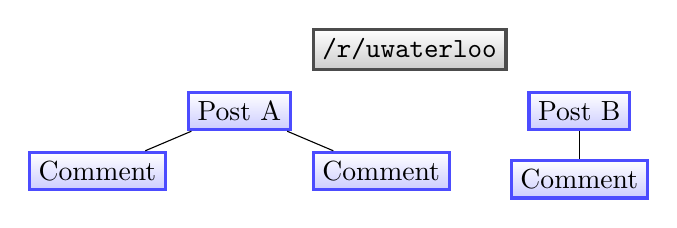
\begin{tikzpicture}[node distance=1em]
    \node (subreddit) [plain] {\texttt{/r/uwaterloo}};
    \node (post_a) [post, below left=of subreddit] {Post A};
    \node (post_b) [post, below right=of subreddit] {Post B};
    \node (comment_1) [post,below left=of post_a] {Comment};
    \node (comment_2) [post,below right=of post_a] {Comment};
    \node (comment_3) [post,below = of post_b] {Comment};

    \path (post_a) edge[-] (comment_1)
          (post_a) edge[-] (comment_2);
    \path (post_b) edge[-] (comment_3);

  \end{tikzpicture}
  \caption{Graph-like structure of the Reddit platform.}
  \label{fig:model:reddit}
\end{figure}

\subsection{Graph Model}
We model the influence model on a given subreddit as a connection between two graphs. A visualization of the structure can be found in Figure~\ref{fig:model:hypergraph}. Graph \(G_P\) is the graph that captures the inherent structural relationship between submissions/comments. Assumptions~\ref{assume:1} and~\ref{assume:2} imply that a given submission is influenced by its comments. More generally, any parent content is directly influenced by its children. These are visualized as the blue edges in Figure~\ref{fig:model:hypergraph}.

\begin{figure}
  \centering
  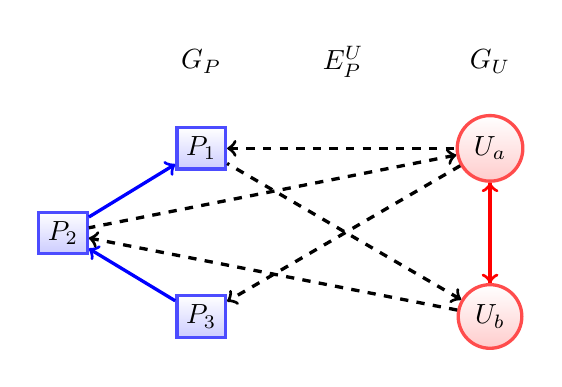
\begin{tikzpicture}[node distance=1em]
    \matrix[row sep=1em, column sep=3em] {
      & \node {$G_P$};& \node {$E_P^U$}; & \node {$G_U$};\\
      & \node (post_a) [post] {$P_1$}; & & \node (user_a) [user] {$U_a$};\\
      \node (comment_1) [post] {$P_2$}; & & & \\
      & \node (comment_2) [post] {$P_3$}; & &\node (user_b) [user] {$U_b$};\\
    };

    \path (post_a) edge[<-, blue, very thick] (comment_1)
          (comment_1) edge[<-, blue, very thick] (comment_2);

    \path (post_a) edge[<-, dashed, very thick] (user_a);
    \path (user_b) edge[<-, dashed, very thick] (post_a)
          (user_b) edge[->, dashed, very thick] (comment_1);
    \path (user_a) edge[<-, dashed, very thick] (comment_1)
          (user_a) edge[->, dashed, very thick] (comment_2);

    \path (user_a) edge[<-, red, very thick] (user_b)
          (user_a) edge[->, red, very thick] (user_b);
  \end{tikzpicture} 
  \caption{Graph structure showing the relationship between users and submissions/comments. \(G_P\) are those nodes and edges that are blue. \(G_U\) are those nodes and edges that are red. \(E_P^U\) is the set of edges denoted by broken lines.}
  \label{fig:model:hypergraph}
\end{figure}
Denote the set of users by \(U\) and the set of submissions and comments by \(P.\) We first define the existence of the digraph \(G_P=(P,E_P)\) that denotes the relationship between submissions and comments. \(E_P\) is constructed in the manner described in Algorithm~\ref{alg:ep}.
\begin{algorithm}
  \For{$parent \in P$}{
    \For{ $child \in P \cap C(P)$ }{
      put directed edge $(child, parent)$ into $E_P$\;
    }
  }
  \caption{Constructing \(E_P\)}
  \label{alg:ep}
\end{algorithm}
We give edges in \(E_P\) a universal weight of \(1.\) Weighting using upvotes was considered but was determined to yield results that were not desireable. For one, it was not clear that upvotes were a meaningful method of ranking influence. Further complexity arises when considering controversial content, which has a mix of upvotes and downvotes. A highly controversial topic may be highly influential, which contradicts the idea that upvotes correlate with influence. Possibly given knowledge of the number of voters this problem could be alleviated. However, since not all subreddits release data about how many users voted, it is simpler to reduce the complexity by eliminating any non-trivial weighting method. Observe that \(G_P\) is a forest where the submissions act as roots of the trees.

This structure by itself is not interesting. We now generate a set of edges \(E_P^U\) that connect submissions/comments to users. 

and \(G_U=(U,E_U,W_U)\) in the following manner.

\section{IMPLEMENTATION}

\section{CONCLUSIONS}

A conclusion section is not required. Although a conclusion may review the main points of the paper, do not replicate the abstract as the conclusion. A conclusion might elaborate on the importance of the work or suggest applications and extensions. 

\addtolength{\textheight}{-12cm}   % This command serves to balance the column lengths
                                  % on the last page of the document manually. It shortens
                                  % the textheight of the last page by a suitable amount.
                                  % This command does not take effect until the next page
                                  % so it should come on the page before the last. Make
                                  % sure that you do not shorten the textheight too much.

%%%%%%%%%%%%%%%%%%%%%%%%%%%%%%%%%%%%%%%%%%%%%%%%%%%%%%%%%%%%%%%%%%%%%%%%%%%%%%%%



%%%%%%%%%%%%%%%%%%%%%%%%%%%%%%%%%%%%%%%%%%%%%%%%%%%%%%%%%%%%%%%%%%%%%%%%%%%%%%%%



%%%%%%%%%%%%%%%%%%%%%%%%%%%%%%%%%%%%%%%%%%%%%%%%%%%%%%%%%%%%%%%%%%%%%%%%%%%%%%%%
\section*{APPENDIX}

Appendixes should appear before the acknowledgment.

\section*{ACKNOWLEDGMENT}

The preferred spelling of the word ÒacknowledgmentÓ in America is without an ÒeÓ after the ÒgÓ. Avoid the stilted expression, ÒOne of us (R. B. G.) thanks . . .Ó  Instead, try ÒR. B. G. thanksÓ. Put sponsor acknowledgments in the unnumbered footnote on the first page.\cite{IEEEExample:IEEEwebsite}



%%%%%%%%%%%%%%%%%%%%%%%%%%%%%%%%%%%%%%%%%%%%%%%%%%%%%%%%%%%%%%%%%%%%%%%%%%%%%%%%
\bibliography{IEEEabrv,root.bib}

\end{document}
